\chapter{Introduction}
\section{Multipath in Aeronautical Telemetry}
Multipath interference is one of the dominant causes for link loss in aeronautical telemetry.
Strong multipath interference occurs in aeronautical telemetry when the transmitted signal is received via multiple paths because a test article is in a low elevation angle scenario as shown in Figure \ref{fig:multipath}.
Multipath propagation is modeled as linear, time-invariant system with a finite impulse response.
Equalizers have been studied to combat multipath interference in aeronautical telemetry \cite{rice-afran-saquib:2014,rice-afran-saquib-cole-rhodes-moazzami:2014}.
There are two types of equalizers, blind and data-aided.
Blind equalizers combat multipath using known properties of the transmitted signal but no knowledge of the data or multipath channel.
Data-aided equalizers require knowledge of the propagation conditions.
One method of obtaining an estimate of this knowledge is to periodically insert a known bit sequence called a ``pilot'' into the data stream.
The receiver compares the received signal corresponding to the pilot with a locally stored copy of the pilot to estimate parameters such as the multipath channel, frequency offset, phase offset, and noise variance.
Data-aided equalizers are finite-length impulse response (FIR) filters. The impulse response of the equalizer filter is computed using the estimated channel.
\begin{figure}
	\centering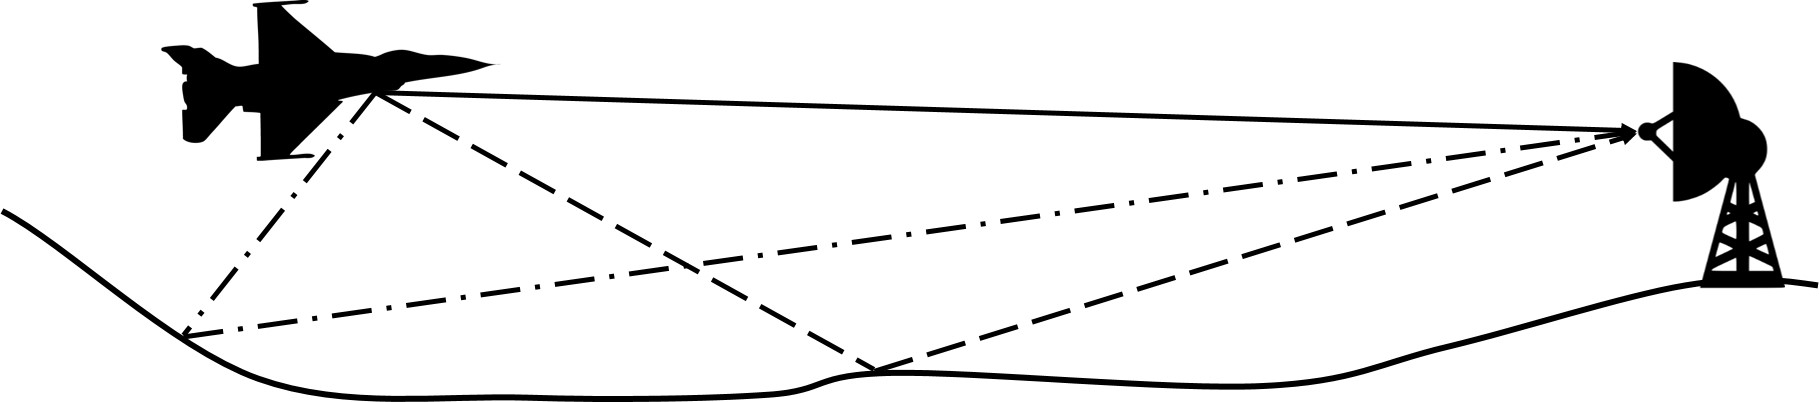
\includegraphics[width=12.11in/100*50]{figures/intro/Picture1.jpg}
	\caption{Multipath can occur when a signal is received multiple paths like line-of-sight or ground bounce or reflections.}
	\label{fig:multipath}
\end{figure}
\section{Problem Statement}
The real-time signal processing for a digital communications system with data-aided equalizers is computationally heavy.
Digital communication algorithms implemented in a high powered Central Processing Unit (CPU) cannot meet the real-time requirement.
Graphic Processing Units (GPUs) can be used to perform real-time processing because of their massively parallel architecture.

This thesis studies how signal processing can be reformulated to run quickly and efficiently in GPUs.
Optimized libraries harness GPU resources to make signal processing implementation relatively easy and extremely fast.
%Processing signals in batches to introduce more parallelism.
If algorithms can be reformulated for batch processing and use matrix/vector multiplication or Fast Fourier Transform libraries, GPUs can provide vast speed ups.

\section{Organization}
Chapter \ref{chap:PAQ_project} describes the Preamble Assisted Equalization (PAQ) system and introduce the digital signal processing algorithms.
Chapter \ref{chap:gpu} provides an overview of signal processing in GPUs.
Chapter \ref{chap:equalizers_in_gpus} describes how the five equalizers are implemented in GPUs.
The thesis concludes with the summary and conclusions in Chapter \ref{chap:final_summary}.